\documentclass[a4paper]{article}

\usepackage[brazil]{babel}
\usepackage[utf8]{inputenc}
\usepackage{graphicx}
\usepackage{hyperref}

\title{Trabalho de Metodologia}

\author{Matheus Tenório dos Santos}

\date{\today}

\begin{document}
\maketitle

%----------------------------------------------

\begin{abstract}

Este documento se refere a um trabalho da disciplina de Metodologia Cientifica, o qual se propõe a responder uma pergunta científica presente num artigo escolhido por mim. Esta resposta se dará pela revisão bibliográfica dos atigos citados pelo artigo escolhido e pelos artigos que citaram o artigo escolhido.

\end{abstract}

%----------------------------------------------

\section{Registros obrigatórios}


\begin{figure}[!h]
	\centering
	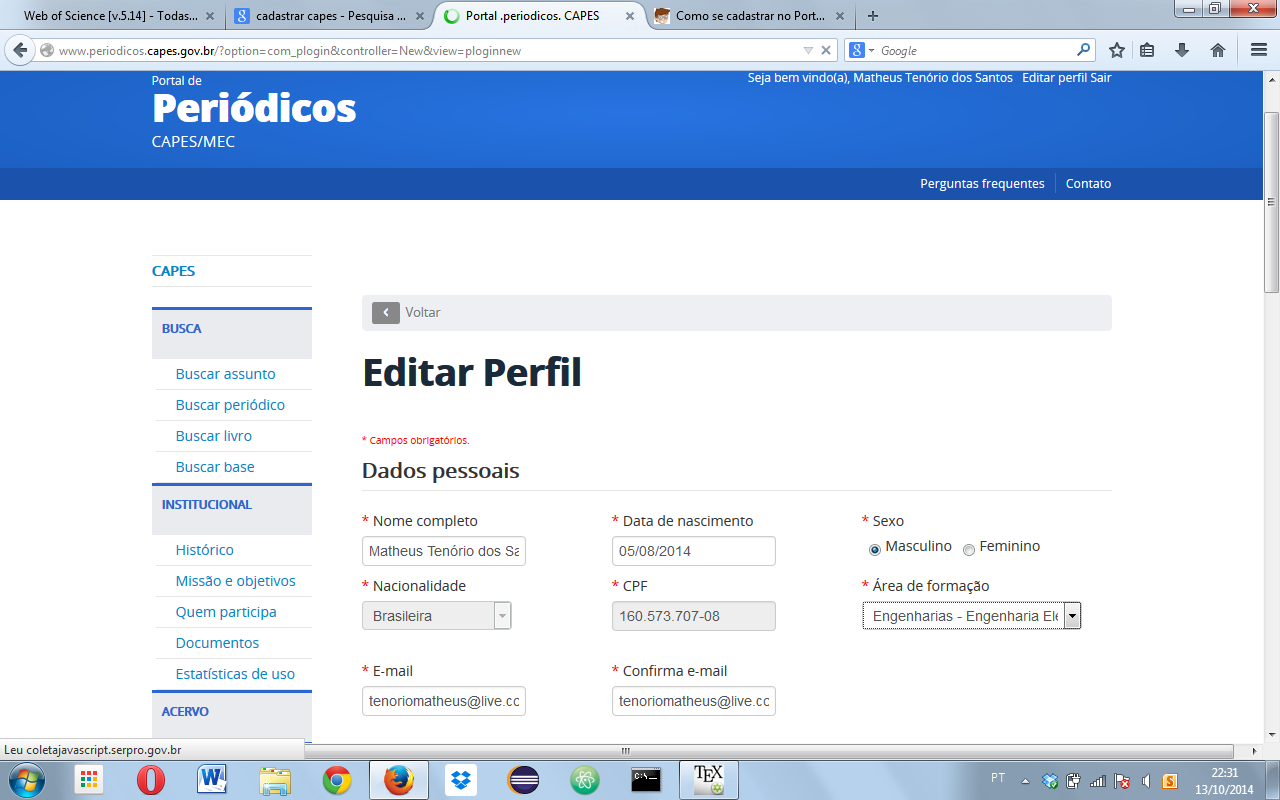
\includegraphics[width=.3\linewidth]{capes.png}
	\caption{\href{./capes.png}{Registro Capes}}
	\label{fig:capes}
\end{figure}

\begin{figure}[!h]
	\centering
  	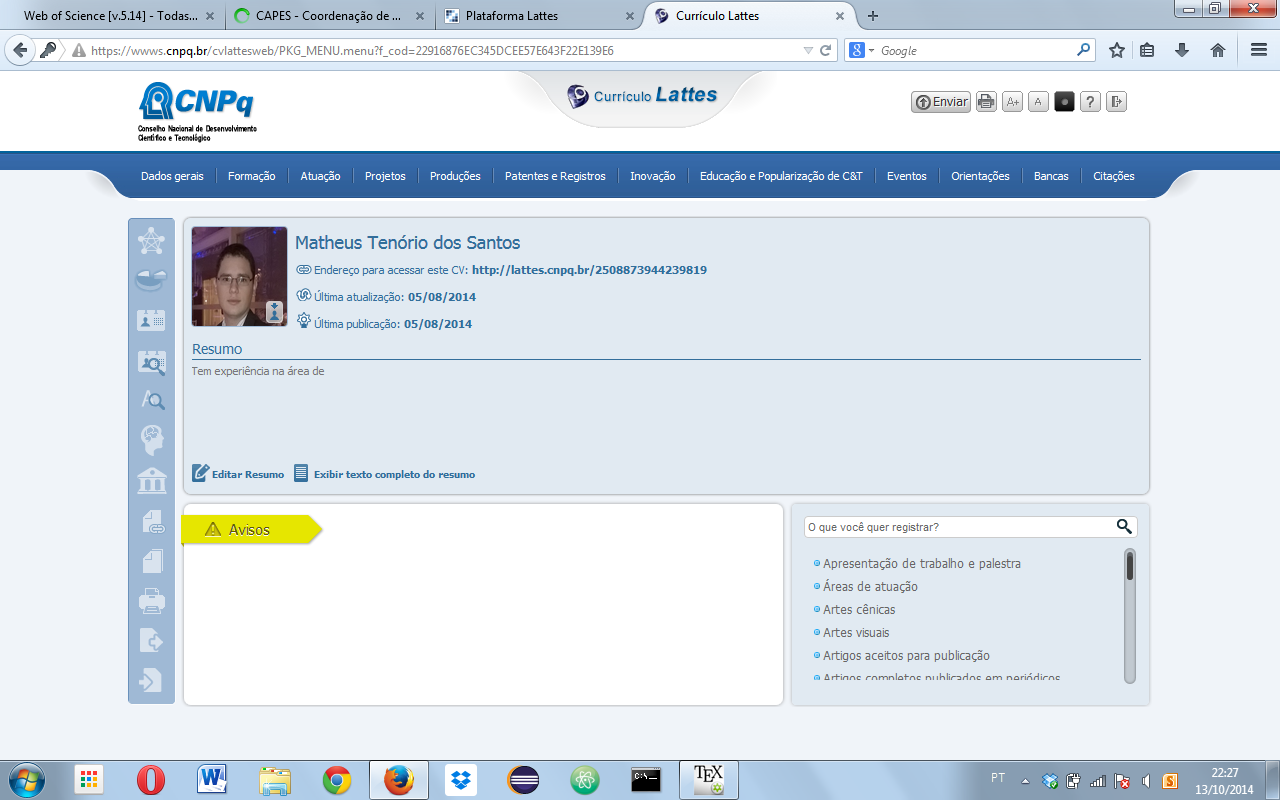
\includegraphics[width=.3\linewidth]{lattes.png}
  	\caption{\href{./lattes.png}{Registro Lattes}}
  	\label{fig:lattes}
\end{figure}

\begin{figure}[!h]
	\centering
	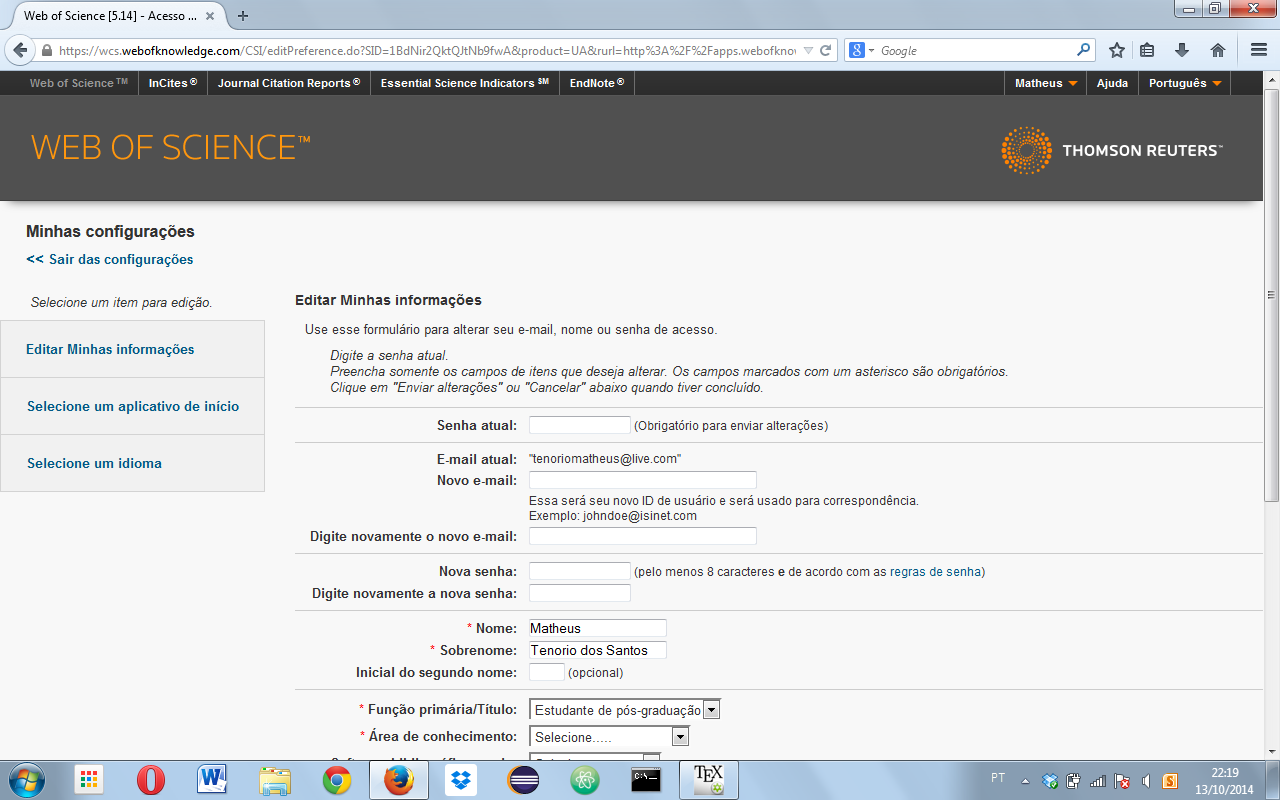
\includegraphics[width=.3\linewidth]{ISI.png}
	\caption{\href{./ISI.png}{Registro ISI}}
	\label{fig:ISI}
\end{figure}

%----------------------------------------------

\section{Pergunta científica}

Quais são os algoritimos de busca espacial mais eficientes até 1995?

%----------------------------------------------

\section{Revisão Bibliográfica}
Os seguintes artigos são capazes de responder a pergunta científica proposta.
\vspace{3mm}

\subsection{1º artigo}

Este artigo \cite{Korf1995} aborda diversos algorítimos de busca espacial. Ele mostra os algorítimos em ordem crescente do mais ineficiente para o mais eficiente. Entre os algorítimos citados estão:

\begin{itemize}

\item Busca por profundidade;
\item Busca por largura;
\item Dijkstra's;
\item A*;
\item Aprofundamento iterativo;
\item Aprofundamento-iterativo-A* (IDA*);
\item Node Retraction;
\item Busca de perímetro (Perimeter Search).

\end{itemize}

\subsection{2º artigo}

Este artigo \cite{Chakrabarti1989} mostra dois algoritimos de busca que são eficientes
quando se possui pouca memória disponivel. Os dois algoritimos são:

\begin{itemize}

\item MA* - para grafos comuns);
\item MAO* - para grafos AND/OR.

\end{itemize}

\subsection{3º artigo}

O terceiro artigo \cite{Korf1993} mostra uma solução para a quantidade de nós gerados pelos
seguintes algoritimos:

\begin{itemize}

\item Busca por largura;
\item Dijkstra;
\item A*.

\end{itemize}

O autor apresenta o algoritimo \' linear-space best-first search' (RBFS) como esta solução. Este algoritimo reduz o número de nós gerados da ordem exponencial para a ordem linear.

\subsection{4º artigo}

\cite{Dillenburg1994}

\begin{itemize}

\item

\end{itemize}

%----------------------------------------------

\bibliographystyle{plain}
\bibliography{bibliografia}

%----------------------------------------------

\end{document}